%!TEX root = ../index.tex
In diesem Kapitel wird die Situation wie sie vor dieser Arbeit war beschrieben.
Es wurde bewusst auf darauf verzichtet Systeme und Gegebenheiten abzudecken,
welche entweder kein Benutzermanagement aufweisen oder nicht von einem grossen
Teil der Mitarbeiter eingesetzt wird.

\section{Systeme mit Benutzermanagement}
\label{sec:Systeme mit Benutzermanagement}

\subsection{Google-Apps}
\label{subs:Google-Apps}
Allink verwendet aus Google-Apps folgende Tools. 
\begin{itemize}
	\item Google Mail 
	\item Google Calendar 
	\item Google Sites 
	\item Google Docs 
	\item Google Analytics 
\end{itemize}

\subsection{Basecamp}
\label{subs:Basecamp}
Mit Basecamp werden Milestones und Todo-Listen für sämtliche Projekte
verwaltet. Zudem werden sämtliche Arbeitsaufwände darin erfasst um am Ende
eines Projekts einen Überblick über alle Arbeitsleistungen zu haben.

\subsection{Mac OS X Server}
\label{subs:Mac OS X Server}

\section{Mitarbeiter}
\label{sec:Mitarbeiter}
Um herauszufinden welche Benutzerdaten die Mitarbeiter kennen und welche
Systeme sie nur verwenden können da das Passwort gespeichert wurde, wurde
mit einer Umfrage der Sachverhalt erörtert.

\begin{tabular}
	{|l | c|} \hline System & Anzahl\\
	\hline Google-Apps & 10\\
	\hline Basecamp & 5\\
	\hline Mac OS X Server & 4\\
	\hline 
\end{tabular}

\section{Login Prozess}
\label{sec:Login Prozess}

\begin{figure}[H]  
		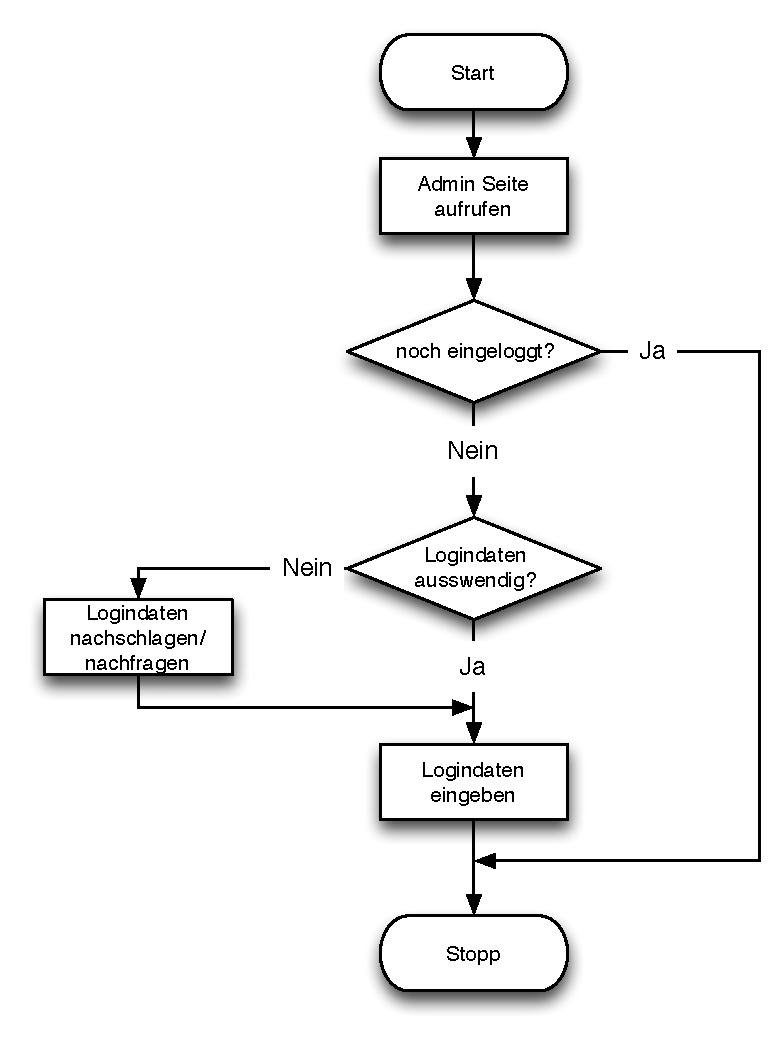
\includegraphics[width=0.70\textwidth]{include/login_before.pdf}
		\caption{Login Prozess vor dieser Arbeit}
		\label{fig:login-before}
\end{figure}
